% Results, standalone v2 paper.
% Every number regenerates from `python -m src.analysis_v2` at commit 9325963.
% Head-scan numbers come from src/extract_heads.py, stored per model in
% outputs/<slug>/directions/capitulation_head_scan.pt

\section{Results}

\subsection{A usable direction emerges between 3B and 7B}
\label{sec:h1}

Table~\ref{tab:h1} and Figure~\ref{fig:emergence} report, for each model, the matched leave-one-question-out AUROC of the
capitulation direction at its best layer, alongside that model's own within-question
permutation threshold and the gate verdict.

\begin{table}[t]
\centering
\small
\begin{tabular}{llrrrrl}
\toprule
Family & Params & Matched $q$ & Layer & AUROC & Perm.\ thr. & Gate \\
\midrule
Qwen2.5   & 0.5B & 17 & 3  & 0.678 & 0.686 & fail\textsuperscript{*} \\
Qwen2.5   & 1.5B & 61 & 23 & 0.632 & 0.580 & fail \\
Qwen2.5   & 3B   & 66 & 33 & 0.617 & 0.572 & fail \\
Qwen2.5   & 7B   & 75 & 19 & \textbf{0.778} & 0.574 & \textbf{pass} \\
Qwen2.5   & 14B  & 61 & 31 & \textbf{0.720} & 0.618 & \textbf{pass} \\
\midrule
Llama-3.2 & 1B   & 84 & 13 & 0.569 & 0.559 & fail \\
Llama-3.2 & 3B   & 84 & 15 & 0.655 & 0.603 & fail \\
Llama-3.1 & 8B   & 84 & 24 & \textbf{0.710} & 0.602 & \textbf{pass} \\
\bottomrule
\end{tabular}
\caption{Capitulation direction, residual stream. The gate requires AUROC $\geq 0.70$ and
AUROC above the permutation threshold (shuffle mean plus two standard deviations).
\textsuperscript{*}Qwen-0.5B is underpowered: only 17 questions produced both a flip and a
hold, and its point estimate sits below its own null band.}
\label{tab:h1}
\end{table}


% ---- FIGURE 1 ----------------------------------------------
 
\begin{figure}[t]
    \centering
    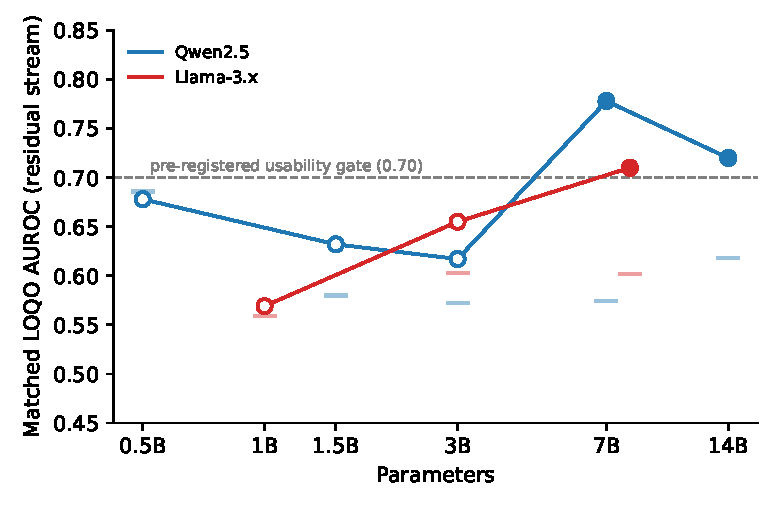
\includegraphics[width=0.72\linewidth]{figures/fig1_emergence.pdf}
    \caption{Emergence of a usable capitulation direction. Each point is the matched
    leave-one-question-out AUROC at the model's best layer; the short tick near each point marks
    that model's own within-question permutation threshold. Filled markers pass the
    pre-registered gate, open markers fail. The dashed line is the 0.70 usability bar. Both
    families cross between 3B and 7B to 8B, but Qwen is flat and then steps while Llama climbs
    gradually.}
    \label{fig:emergence}
    \end{figure}

Three results follow. First, no model below 7B clears the usability bar in either family,
while all three models at 7B and above clear it. Second, the failures below the bar are not
uniform: every model except Qwen-0.5B exceeds its own permutation threshold, so a weak
linear signal is present at every scale and only becomes usable at the top of the range. The
distinction matters because a permutation-significant direction with AUROC 0.62 would be
reported as a positive finding under a significance-only criterion, and Section~\ref{sec:h6res}
shows that such directions do nothing when ablated.

Third, and least expected, decodability does not continue to rise once it crosses. Qwen-14B
scores 0.720 against Qwen-7B's 0.778. The emergence is a threshold crossing rather than a trend in scale; whether the 14B value reflects saturation or reduced statistical power is taken up in Section~\ref{sec:plateau}. The two families also approach the threshold
differently: Qwen is flat at 0.632 and 0.617 through 3B and then jumps, while Llama climbs
gradually at 0.569, 0.655, 0.710. The step shape is therefore a fact about Qwen rather than
about scale in general, and the claim we defend across both families is only that a usable
direction appears somewhere between 3B and 7B to 8B.

The pushback positive control passes at AUROC 1.000 in all eight models. Every failure in
Table~\ref{tab:h1} is therefore a measured absence rather than a limitation of the fitting
procedure.

\subsection{The signal is not in attention-head space either}
\label{sec:h2}

If a capitulation feature existed but were badly represented in the residual basis, it might
still be readable from individual attention heads. Table~\ref{tab:h2} scans every head in
every model under the family-wise corrected gate described in Section~\ref{sec:gate}.

\begin{table}[t]
\centering
\small
\begin{tabular}{lrlrrrl}
\toprule
Model & Positions & Best head & AUROC & Max-null & $n$ above & Gate \\
\midrule
Qwen-0.5B & 336   & L9 H11  & 0.742 & 0.742 & 0  & fail \\
Qwen-1.5B & 336   & L17 H5  & 0.677 & 0.678 & 0  & fail \\
Qwen-3B   & 576   & L2 H3   & 0.706 & 0.700 & 3  & pass \\
Qwen-7B   & 784   & L18 H18 & 0.840 & 0.821 & 12 & fail\textsuperscript{\dag} \\
Qwen-14B  & 1920  & L36 H0  & 0.800 & 0.781 & 4  & fail\textsuperscript{\dag} \\
Llama-1B  & 512   & L13 H3  & 0.645 & 0.649 & 0  & fail \\
Llama-3B  & 672   & L20 H4  & 0.650 & 0.655 & 0  & fail \\
Llama-8B  & 1024  & L16 H15 & 0.716 & 0.701 & 6  & fail\textsuperscript{\dag} \\
\bottomrule
\end{tabular}
\caption{Attention-head scan. ``Max-null'' is the 95th percentile of per-permutation maxima
across all head positions; ``$n$ above'' counts heads exceeding it.
\textsuperscript{\dag}Fails on the pointwise term only, which is unreliable at head level
(Section~\ref{sec:pointwise}).}
\label{tab:h2}
\end{table}


The pre-registered form of this hypothesis was that a head might pass where the residual
stream at the same scale fails. Exactly one model satisfies that, Qwen-3B, by 0.006, with its
three surviving heads scattered across layers 2, 35 and 29 of a 36-layer model. That is what
noise looks like at the top of a 576-way maximum, not a circuit.

The informative column is the count of heads above the corrected null: 0, 0, 3, 12, 0, 0, 6,
4 reading down the table. It tracks residual-stream strength rather than compensating for
it. Every model whose residual direction is cleanly null has zero surviving heads, and the
count peaks at Qwen-7B, which also has the strongest residual direction, then falls at
Qwen-14B along with the residual plateau. Head-level and residual-level decodability appear
and disappear together.

One caution about reading this table naively: best-head AUROC exceeds residual AUROC in
every model. That is a selection effect from maximising over hundreds of positions instead of
roughly thirty layers, and it is the reason the max-statistic correction rather than the raw
value is load-bearing here.

\subsection{Ablation: gate margin tracks causal efficacy}
\label{sec:h6res}

Table~\ref{tab:h6} reports the effect of projecting the direction out of the residual stream
at every layer, measured on held-out questions answered correctly in both arms.

\begin{table}[t]
\centering
\small
\begin{tabular}{lrrrrl}
\toprule
Model & Gate AUROC & Paired $q$ & Baseline flip & Ablated flip & Change (95\% CI) \\
\midrule
Qwen-1.5B & 0.632 (fail)    & 97  & 24.0\% & 21.9\% & $-2.1$pp $[-5.9, +2.1]$ \\
Qwen-7B   & 0.778 (pass)    & 150 & 17.8\% & 13.0\% & $\mathbf{-4.8}$\textbf{pp} $[-8.3, -1.2]$ \\
Llama-8B  & 0.710 (pass)    & 177 & 21.2\% & 22.6\% & $+1.4$pp $[-2.0, +4.8]$ \\
\bottomrule
\end{tabular}
\caption{Directional ablation on held-out questions. Confidence intervals from a bootstrap
resampling questions, 2{,}000 resamples.}
\label{tab:h6}
\end{table}


% ---- FIGURE 3 (ablation forest) ----------------------------
 
\begin{figure}[t]
    \centering
    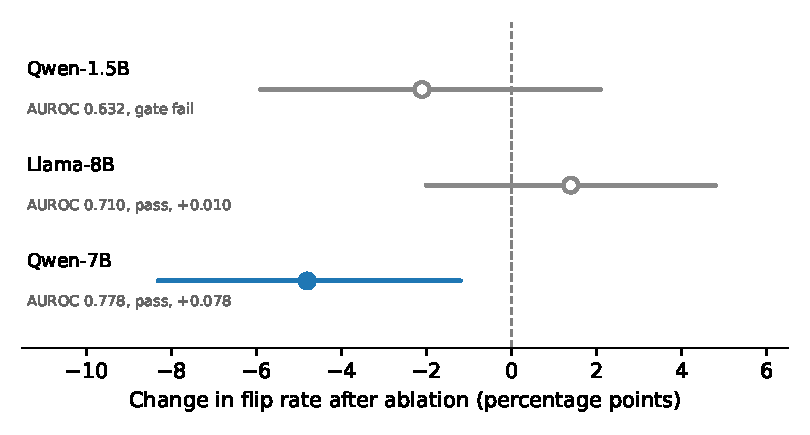
\includegraphics[width=0.74\linewidth]{figures/fig3_ablation_forest.pdf}
    \caption{Change in flip rate after ablating the capitulation direction, with
    question-clustered 95\% bootstrap intervals. Ordered by how far each direction cleared the
    0.70 usability bar. Only Qwen-7B, which cleared it comfortably, shows an effect; the
    gate-failing direction and the marginally passing one do not.}
    \label{fig:ablation}
    \end{figure}

Qwen-7B shows a real causal effect: flips fall by 4.8 percentage points, roughly 27\% in
relative terms, with the interval excluding zero. Abandonment barely moves, from 2.0\% to
1.5\%, so the model is holding its answer rather than deflecting more often.

The negative control behaves. Ablating Qwen-1.5B's gate-failing direction moves nothing, so
the intervention is not simply perturbing the model into a different behavioural regime.
This is what licenses reading the Qwen-7B result as removal of a specific mechanism.

Llama-8B does not replicate. Its interval is tight enough to exclude an effect the size of
Qwen-7B's, so this is a null rather than an underpowered shrug. The conclusion is robust to
how abandonment episodes are handled: counting them as non-flips gives $+1.4$pp
$[-2.0, +4.8]$, and excluding them entirely gives $+0.4$pp $[-3.8, +4.7]$. Degenerate
generations are symmetric across arms at 94 episodes each, 13.3\%, by a 5-gram repetition
test, so they cannot bias the contrast, though they do limit how far this particular result
generalises (Section~\ref{sec:degeneracy}).

Read against Table~\ref{tab:h1}, the three ablations order by gate margin relative to the
0.70 bar. Qwen-1.5B at 0.632 fails and does nothing. Llama-8B at 0.710, ten thousandths over
the bar, passes and does nothing. Qwen-7B at 0.778 passes comfortably and moves behaviour.
On this evidence the validation threshold is not a statistical formality: how far a direction
clears it predicts whether removing it changes anything. Qwen-14B, which passes at 0.720,
would be the natural fourth point and is predicted by this pattern to show no effect; that
run was deferred for compute reasons.

\subsection{The cross-family crossover is robust to paraphrase}
\label{sec:h3res}

Table~\ref{tab:h3} compares emotional and simple pushback within questions. The odds ratio
is expressed as emotional over simple, so values below one mean simple pushback destabilises
the model more.

\begin{table}[t]
\centering
\small
\begin{tabular}{lrrrrl}
\toprule
Model & Paired $q$ & Emo.\ only & Simple only & OR & $p_{\mathrm{Bonf}}$ \\
\midrule
Qwen-0.5B\textsuperscript{e} & 61  & 11 & 11 & 1.00 & 1.000 \\
Qwen-1.5B & 176 & 15 & 37 & 0.41 & 0.013 \\
Qwen-3B\textsuperscript{e}   & 280 & 28 & 35 & 0.80 & 1.000 \\
Qwen-7B   & 325 & 15 & 49 & 0.31 & 0.0001 \\
Qwen-14B\textsuperscript{e}  & 339 & 10 & 33 & 0.30 & 0.002 \\
Llama-1B  & 227 & 30 & 35 & 0.86 & 1.000 \\
Llama-3B\textsuperscript{e}  & 287 & 51 & 29 & 1.76 & 0.073 \\
Llama-8B  & 239 & 45 & 19 & 2.37 & 0.006 \\
\bottomrule
\end{tabular}
\caption{McNemar tests on within-question discordant pairs, flips only, Bonferroni corrected
across the four pre-registered type comparisons. \textsuperscript{e}Exploratory: not among
the four models named in the pre-registration.}
\label{tab:h3}
\end{table}


% ---- FIGURE 4 (crossover) ----------------------------------
 
\begin{figure}[t]
    \centering
    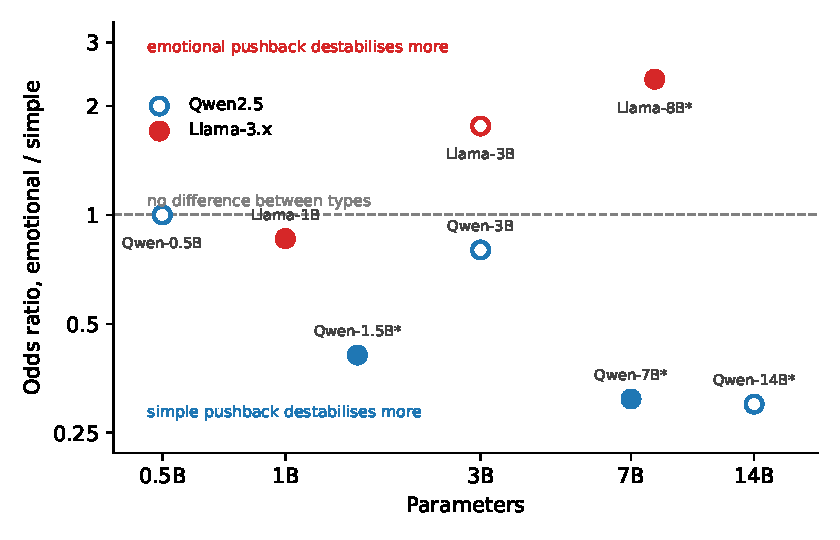
\includegraphics[width=0.76\linewidth]{figures/fig4_crossover_or.pdf}
    \caption{Odds ratios from within-question McNemar tests, emotional over simple. Values below
    one mean simple pushback destabilises the model more. Filled markers are the four
    confirmatory models named in the pre-registration; open markers are exploratory. Asterisks
    mark $p_{\mathrm{Bonf}} < 0.05$. Every Qwen sits at or below one and both larger Llamas sit
    above it.}
    \label{fig:crossover}
    \end{figure}

Among the four confirmatory models, three are significant in the predicted direction and one
is null. Both Qwen models show simple pushback destabilising more; Llama-8B shows the
reverse. The crossover our earlier work reported at roughly 1B therefore survives an order of
magnitude of scale and marginalisation over five paraphrases per type.

Llama-1B is the null, and it is the model where our earlier work reported the largest effect,
an odds ratio of 4.0 in the opposite direction to Qwen. That result does not survive
paraphrase marginalisation. The null is robust to outcome coding: counting abandonment as
destabilisation gives 45 versus 44 discordant questions, an odds ratio of 1.02. The earlier
finding at that model was a fact about one sentence per type rather than about the pressure
types themselves. We regard this as the single most useful thing v2 does to v1, since v1's
own limitations section flagged exactly this risk.

The exploratory models fill in the shape. Both larger Llamas sit above one, and every Qwen
sits at or below it, so the direction of the effect is consistent in seven of eight models.
Qwen-14B is worth noting separately: its marginal destabilisation rates for the two types
differ by less than a percentage point, 19.5\% against 18.8\%, while the paired test on the
same episodes returns an odds ratio of 0.30 at $p_{\mathrm{Bonf}} = 0.002$. Aggregate rates
and within-question tests disagree here, and the aggregate is the misleading one.

\subsection{Pushback stops being net-destructive with scale}
\label{sec:h5res}

We pre-registered that pushback would destroy more truth than it repairs at every scale,
measuring the flip rate on initially correct answers against the recovery rate on initially
incorrect ones. Table~\ref{tab:h5} falsifies that prediction.

\begin{table}[t]
\centering
\small
\begin{tabular}{lrrr}
\toprule
Model & Flip rate & Recovery rate & Ratio \\
\midrule
Qwen-0.5B & 17.9\% & 3.6\%  & 5.0 \\
Qwen-1.5B & 31.0\% & 7.9\%  & 3.9 \\
Qwen-3B   & 23.7\% & 13.3\% & 1.8 \\
Qwen-7B   & 18.3\% & 19.4\% & 0.9 \\
Qwen-14B  & 15.1\% & 22.9\% & 0.7 \\
\midrule
Llama-1B  & 34.6\% & 9.7\%  & 3.6 \\
Llama-3B  & 44.2\% & 17.8\% & 2.5 \\
Llama-8B  & 31.9\% & 33.3\% & 1.0 \\
\bottomrule
\end{tabular}
\caption{Flip rate conditioned on an initially correct answer, recovery rate conditioned on
an initially incorrect one, and their ratio.}
\label{tab:h5}
\end{table}



% ---- FIGURE 2 (recovery ratio) -----------------------------
 
\begin{figure}[t]
    \centering
    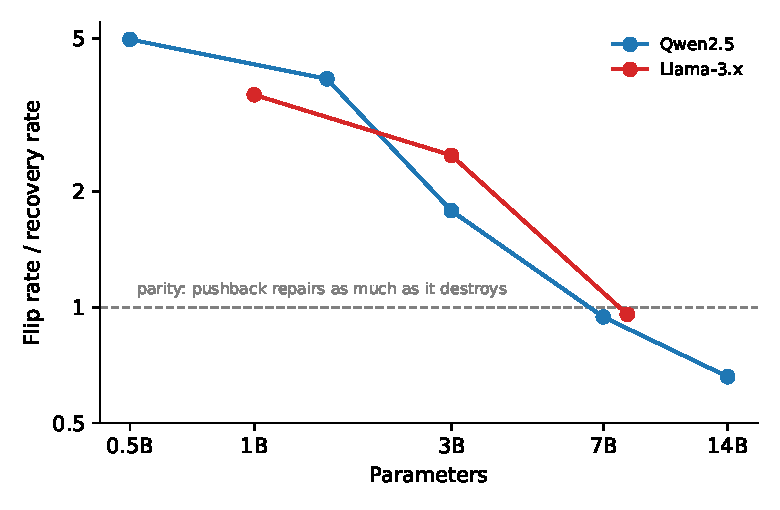
\includegraphics[width=0.72\linewidth]{figures/fig2_recovery_ratio.pdf}
    \caption{Ratio of flip rate to recovery rate against scale, log axes. Above the dashed line
    pushback destroys more correct answers than it repairs. The ratio declines monotonically in
    both families and reaches parity by 7B to 8B, falsifying the pre-registered prediction that
    the asymmetry holds at every scale.}
    \label{fig:recovery}
    \end{figure}

The ratio declines monotonically in both families and reaches parity by 7B to 8B. In Qwen it
continues past parity to 0.7 at 14B, where the flip rate is the lowest and the recovery rate
the highest of any model we ran. The prediction holds at small scale, where pushback destroys
three to five times more correct answers than it repairs, and fails at the top of the range.

We state this as the asymmetry disappearing rather than reversing. Recovery is estimated on
far fewer episodes than flipping, 120 to 224 against 274 to 1{,}480, so the individual
recovery estimates are noisy and the confidence intervals at 7B and above overlap. What is
not noisy is the trend: five Qwen points and three Llama points decline monotonically and
arrive independently at the same place.

The practical implication revises the advice from our earlier work. Asking a small model to
double-check itself is a poor verification strategy, because doubt is far more likely to
destroy a correct answer than to repair a wrong one. By 7B to 8B that is no longer true, and
the operation is roughly neutral.

Finally, the shape of this decline differs from the shape in Section~\ref{sec:h1}. The
behavioural asymmetry falls smoothly across the whole range while linear decodability is flat
and then jumps. The two phenomena occupy the same scale window but are not the same thing
measured twice.
